\def \secname {Solution of problems in two space dimensions}

\section[\secname]{\hyperlink{toc}{\secname}}




Time-dependent equation that we study, diffusion equation, will serve as a model for the solution of the Schroedinger Equation that we will solve in the Project 2.

\subsection{Diffusion Equation}

\begin{itemize}
    \item Model Equation

    \[ y(x,y,t)_t = \nabla ^2 u = u_{xx} + u_{yy}\]

    \[ u_t = u_{xx} + u_{yy} \qquad \sigma = 1\]

    where sigma is the diffusion constant.

    On 

    \[ 0 \le x \le 1, \quad 0 \le y \le 1; \quad t\ge 0\]

    Subject to 

    \[ u(x,y,0) = u_0(x,y)\]

    \[ u(0,y,t) = u(1,y,t) = u(x,0,t) = u(x,1,t) = 0\]

    \item Solve by FDA

    \item Step 1: Discretize Domain

    Spatial Mesh

    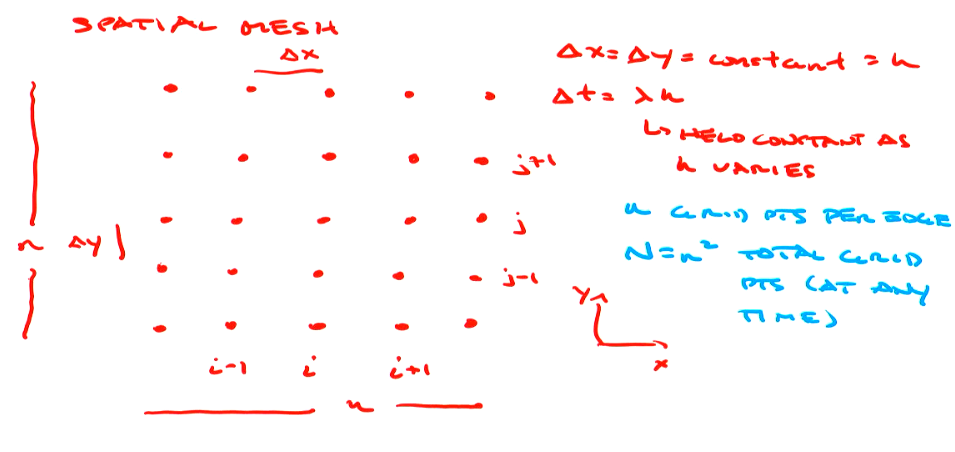
\includegraphics[width  = \linewidth]{Images/2D_spatialmesh_diffusion.png}

    \begin{equation}
        \begin{bmatrix}
            u_{1,1} \\
            \vdots \\
            u_{n,1} \\
            \vdots \\
            u_{1,n} \\
            \vdots \\
            u_{n,n}
        \end{bmatrix} = \mathbf{u}^n \qquad n^2 = N \text{ components}
    \end{equation}
    \item Grid Function notation

    \[ u_{i,j}^n = u(x_i, y_j, t^n)\]
\end{itemize}

\subsection{The Crank-Nicholson Scheme For 2D Diffusion Equation}

\begin{itemize}
    \item Assume retains 1-D properties: second-order accuracy, unconditional stability

    \item Introduce F.D. operators: $\p_{xx}^h$, and $\p_{yy}^h$

    \[ \p_{xx}^h u_{i,j}^n =  \frac{ u^n_{i+1,j} - 2u^n_{i,j}+u^n_{i-1,j}}{\Delta x^2}\]

    \[ \p_{yy}^h u_{i,j}^n = \frac{ u^n_{i+1,j} - 2u^n_{i,j}+u^n_{i-1,j}}{\Delta y^2}\]

    \item Then scheme is 

    \[ \frac{u_{i,j}^{n+1}-u_{i,j}^n}{\Delta t} = \frac{1}{2} ( \p_{xx}^h + \p_{yy}^h ) ( u_{i,j}^{n+1} + u_{i,j}^n)\]

    Centre point of scheme

    \[ (x_i, y_j, t^{n+\frac{1}{2}})\]

    \item Truncation error ($\Delta x = \Delta y$)

    \[ \tau = \frac{1}{24} \Delta t^2 (u_{ttt})_{i,j}^{n+\frac{1}{2}} - \frac{1}{8} \Delta t^2 ((u_{ttxx})_{i,j}^{n+\frac{1}{2}}+ (u_{ttxx})_{i,j}^{n+\frac{1}{2}}) - \frac{1}{12} \Delta x^2 ((u_{xxxx})_{i,j}^{n+\frac{1}{2}} + (u_{yyyy})^{n+\frac{1}{2}}_{i,j}) + O(h^4)\]

    \[ = O(\Delta t^2, \Delta x^2) = O(h^2)\]

    Second order in space and time

    \item Define 

    \[ L^h \equiv \p_{xx}^h + \p_{yy}^h\]

    The scheme can be written as 

    \[ (1- \frac{\Delta t}{2} L^h) u_{i,j}^{n+1} = (1+ \frac{\Delta t}{2} L ^h) u_{i,j}^n\]

    Represents linear system of equations for $u_{i,j}^{n+1}$

    \[ \mathbf{A} \mathbf{u}^{n+1} = \mathbf{b}\]

    Where the u vector is all unknown $u_{i,j}^{n+1}$ arranged row by row E.G.

    \item $\mathbf{A}$ will again be sparse; what is its sparsity structure?

    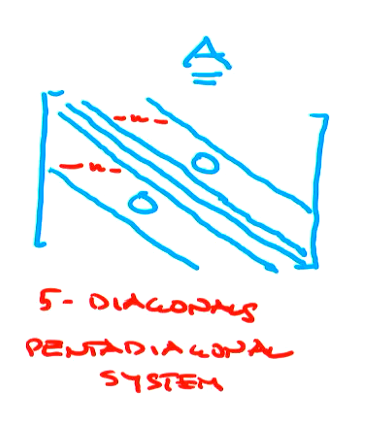
\includegraphics[width = 0.5\linewidth]{Images/pentadiagonal.png}

    Think coupling with nearest neighbour left and right $\pm 1$ and then also above and below $\pm n$ (unlikely to ask this on the final exam)
    
    \item What is cost of solving systems ? (Recall in 1-D we had tridiagonal system, cost was $O(n) = O(N) \Rightarrow$ Optimal); here $O(n^2) = O(N)$ is optimal

    \item Bandwidth, W, of matrix is total number of diagonals that span non-zeros portion

    \item For constant bandwidth NxN systems can be solved in $O(c_w N)$ time when $c_w$ is a constant that depends on $c_w$; $c_w$ is quadratic in $w$

    \textbf{November 8th 2023, 11am}

    \item $c_w \sim n^2$ so the order is still $O(N^2)$ 

    \item $\Rightarrow$ Direct solution of the linear system even taking into account sparsity structure is too expensive

    \item IDEA: operator on left is schematically 

    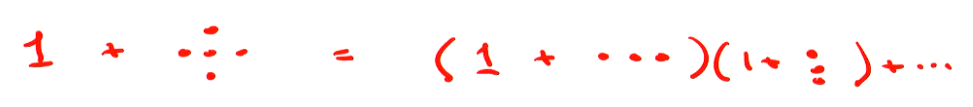
\includegraphics[width = 0.9 \linewidth]{Images/operator_schematic.png}

    
\end{itemize}

\subsection{Altenating direction implicit method for the diffusion equation}

**Hint for Project 2, try this before trying for Project 2** \newline

Factor operator on left into 1-D operators $\Rightarrow$ resulting linear systems are tridiagonal and can be solved efficiently.

\[ (1-\frac{\Delta t}{2} L^h) u_{i,j}^{n+1} = (1+ \frac{\Delta t}{2} L^h) u_{i,j}^{n}\]

\begin{itemize}
    \item Recall: $L^h = \p_{xx}^h + \p_{yy}^h$, so factor

    \[ (1-\frac{\Delta t}{2} \p_{xx}^h)(1-\frac{\Delta t}{2} \p_{yy}^h) u_{i,j}^{n+1} = (1+\frac{\Delta t}{2} \p_{xx}^h)(1+\frac{\Delta t}{2} \p_{yy}^h) u_{i,j}^{n} + \frac{\Delta t^2}{4} \p_{xx}^h \p_{yy}^h (u_{i,j}^{n+1}-u_{i,j}^n)\]

    where the last added term are the quadratic terms from factorization ($O(\Delta t^3)$

    \[ u_{i,j}^{n+1} = u_{i,j}^{n} + \Delta t(u_t)_{i,j}^2 + O(\Delta t^2)\]

    \[ u_{i,j}^{n+1} - u_{i,j}^{n} = O(\Delta t) \]

    So we have

    \[ (\qquad )(\qquad ) u_{i,j}^{n+1} = (\qquad)(\qquad)u_{i,j}^{n} + O(\Delta t^2)\]

    This defines the one-step update $\Rightarrow$ for $O(\Delta t^2)$ global error can neglect $O(\Delta t^2)$ term

    Gives one for of ADI scheme

    \begin{equation}
        (1-\frac{\Delta t}{2} \p_{xx}^h )(1-\frac{\Delta t}{2}\p_{yy}^h) u_{i,j}^{n+1} = (1+\frac{\Delta t}{2} \p_{xx}^h)(1+\frac{\Delta t}{2} \p_{yy}^h) u_{i,j}^{n}
    \end{equation}

    \item Solve in stages: introduce intermediate grid function $u_{i,j}^{n+\frac{1}{2}}$

    let;

    \begin{equation}
        (1-\frac{\Delta t}{2} \p_{xx}^h ) u_{i,j}^{n+\frac{1}{2}} = (1+\frac{\Delta t}{2} \p_{xx}^h)(1+\frac{\Delta t}{2} \p_{yy}^h) u_{i,j}^{n}
    \end{equation}
    
    \begin{equation}
        (1-\frac{\Delta t}{2}\p_{yy}^h) u_{i,j}^{n+1}  = u_{i,j}^{n+\frac{1}{2}} 
    \end{equation}

    \item Key Observation: Each stage requires solution of \~ n tridiagonal systems each of which costs $O(n) \Rightarrow $ total cost $ = O(n^2) - O(N) \Rightarrow$ optimal

    \item Specifically
    \begin{itemize}
        \item Stage 1: for each $j=2,3,\ldots,n-1$ solve tridiagonal systems for $u_{i,j}^{n+\frac{1}{2}}$ from $i=1,2,\ldots, n$

        \item Stage 2: for each $i =2,3,\ldots,n-1$ solve tridiagonal systems for $u_{i,j}^{n+1}$ from $j=1,2,\ldots, n$

        Loops run over $2,3,\ldots,n-1$ since B.C.'s fixed, $u_{i,j}^{n+1}$, does not change in time
    \end{itemize}

    \item Classical version of the ADI method 

    \begin{itemize}
        \item Use fact that $(1+\Delta t \p_{xx}^h/2)^{-1}$ and $(1-\Delta t \p_{xx}^h/2)$  commute to show that the following form is equivalent

        \[ (1-\frac{\Delta t}{2} \p_{xx}^h ) u_{i,j}^{n+\frac{1}{2}} = (1+\frac{\Delta t}{2} \p_{yy}^h) u_{i,j}^{n}\]

        \[ (1-\frac{\Delta t}{2} \p_{yy}^h ) u_{i,j}^{n+1} = (1+\frac{\Delta t}{2} \p_{xx}^h) u_{i,j}^{n+\frac{1}{2}}\]

        Again solved in two stages, each involving tridiagonal solves
    \end{itemize}
\end{itemize}


\textbf{November 10th 2023 - following Kenneth notes}

\subsection{Time-Independent: Solving Elliptic PDEs}

(Elliptic meaning there is no time dependence)

\begin{itemize}
    \item Like 2-point BVPs, but in higher dimension. Let's just look at 2D.
\end{itemize}


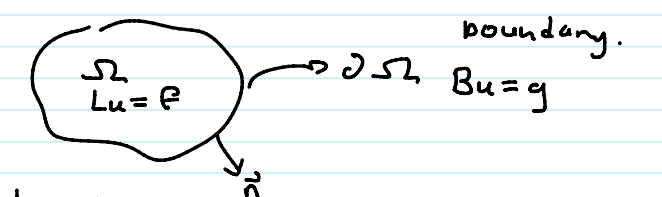
\includegraphics[width = 0.4\linewidth]{Images/elliptic_PDE_setup.png}

\[ \text{Solution domain:} \qquad \Omega\]

\[ \text{Boundary:} \qquad \partial \Omega \]

Look for $u(x,y)$ satisfying

$L u(x,y) = f(x,y)$ on $\Omega$

$L$ -- elliptic differential operator

$f$ -- source/forcing function

$Bu(x,y) = g(x,y)$ on $\partial \Omega$

$B$ -- another operator that encodes BCs

$g$ -- another source function

\vspace{10px}
3 Types of BC's

\begin{enumerate}
    \item Dirichlet - value of u on $\partial R$ is given

    \item Neumann - normal derivative of v on $\partial \Omega $ is given.

    \item Mixed/Robin - some linear combo of $\alpha(x,y)u+\beta (x,y) \frac{\partial u}{\partial x}$ is given.
\end{enumerate}

\subsection{Model Problem}

\begin{itemize}
    \item Poisson equation on unit square with homogeneous Dirichlet Conditions

    \[\nabla ^2 u(x,y) = u_{xx} + u_{yy} = f(x,y) \]

    Subject to 

    \[ u(0,y) = u(1,y) = u(x,0) = u(x,1) = 0\]

    2-1 Discretize Model Problem

    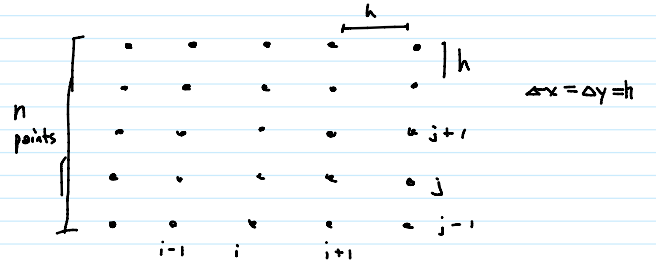
\includegraphics[width = 0.5\linewidth]{Images/model_problem_grid.png}

    \item \textbf{2nd step: }- FDA

    \[ l^h u^h : f^h\]

    \[ B^hu^h: ?\]

    \[ u_{xx} = \frac{u_{i+1,j}-2u_{i,j}+u_{i,j-1}}{h^2} + O(h^2)\]

    \[ u_{yy} = \frac{u_{i+1,j}-2u_{i,j}+u_{i,j-1}}{h^2} + O(h^2)\]

    Substitute into poisson equation

    \[ \frac{u_{i+1,j}+u_{i-1,j}+u_{i,j+1}+u_{i,j-1}-4u{i,j}}{h^2} = f_{i,j} \qquad 2\le i,j\le n-1\]

    where n is the number of points one side

    Discrete BCs
    \[u_{1,j} = u_{n,j} = u_{i,1} = u_{i,n} = 0\]

    using the `plus' stencil

    note that the corner points (0,0), (n,0), (0,n), (n,n) are completely separate due to our stencil choice. But it may be more convenient to just incorporate the points.


    \item \textbf{3rd Step:} How do we solve these equations?

    Write as a linear system

    \[ \mathbf{A} \mathbf{u} = \mathbf{b}\]

    where A has the same sparsity structure as from RD diffusion. Also, its direct solution is expensive, even when accounting for sparsity structure.

    \item Can't us ADI, since (apparently) we can't factor operator into (1-m)(1+m)

    \item A: Use method of relaxation

    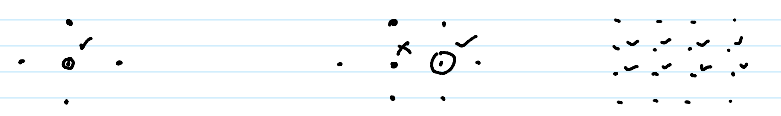
\includegraphics[width = 0.7 \linewidth]{Images/relaxation_stencils.png}
    \begin{enumerate}
        \item plus shape: Instanteously satisfy equation for centerpoint

        \item 2nd one: Move right and satisfy the equation for the next point. Will unsatisfy the previous point in the process! 

        \item large rectangle: Keep going with kick, we get a good solution despite the unsatisfactions (Gauss used this)
    \end{enumerate}
    
\end{itemize}

In his words

\begin{itemize}
    \item Visit each unknown in grid in some order, (row by row, column by column).

    Fix/Freeze other unknowns, adjust our unknown so that its equation is `instantaneously' satisfied.

    \item One complete pass through grid = a relaxation sweep
\end{itemize}

Under certain conditions, this solution will converge.

2 Main ways to update

\begin{enumerate}
    \item Jacobian - use unknowns from previous iteration to satisfy local equations.
    \item Gauss-Seidel - use unknowns most recently computed iteration
\end{enumerate}

We will go over Gauss-Seidel.

\begin{itemize}
    \item Faster
    \item better storage efficiency
    \item basis for successive over relaxation
\end{itemize}

Will also go over way that generalizes immediately to nonlinear equations

Let:

\[ u_{i,j}^{(n)} = \text{discrete solution approx to } u_{i,j} \text{at nth iteration (sweep)} \]

here we assume i sweeps most rapidly

\begin{verbatim}
    for j= 1:n
        for i = 1:n % not those exact indices since only sweeping interior points
\end{verbatim}

\textbf{Residual}

\[ r_{i,j}^{(n)} = h^{-2}(u_{i-1,j}^{(n+1)} + u_{i+1,j}^{(n)} + u_{i,j-1}^{(n+1)}+u_{i,j+1}^{(n)}-4u_{i,j}^{(n)})-f_{i,j}\]

Updates i (right) direction first and then j (up) direction second. This explains the different n-indices in the residual equation.

\textbf{November 17th 11am}

Model Problem (ignoring B.C.'s)

\[ u_{xx} + u_{yy} = f(x,y) \qquad u = u(x,y)\]

Residual for GS relaxation sweep

\[ r_{i,j}^(n) = h^{-2}(u_{i-1,j}^{(n+1)} + u_{i+1,j}^{(n)} + u_{i,j-1}^{(n+1)}+u_{i,j+1}^{(n)}-4u_{1,j}^{(n)})-f_{i,j}\]


\begin{itemize}
    \item Write relaxation in terms of update $\delta u_{i,j}^{(n)}$ and in a way that immediately generatlizes to nonlinear case.

    \[ u_{i,j}^{(n)} \rightarrow u_{i,j}^{(n+1)} = u_{i,j}^{(n)} - r u_{i,j}^{(n)}\]

    \item First define 

    \[ F_{i,j}^h = \frac{u_{i+1,j} + u_{i-1,j}+u_{i,j+1}+u_{i,j-1}-4u_{i,j}}{h^2}-f_{i,j}\]

    \item Newton's Method 

    \[ u_{i,j}^{(n+1)} = u_{i,j}^{(n)} - r_{i,j}^{(n)} \left[ \left. \frac{\partial F_{i,j}^h}{\partial u_{i,j}} \right|_{u_{i,j} = u_{i,j}^{(n)}} \right]^{-1}\]

    \[ u_{i,j}^{(n)} - \frac{r_{i,j}^{(n)}}{-4h^{-2}}\]

    \[ = u_{i,j}^{(n)} + \frac{1}{4} h^2 r_{i,j}^{(n)}\]

    \item Equation above is equivalent to solving other equation directly for $u_{i,j}$ (verify)
\end{itemize}

\subsection{Convergence of Relaxation Methods}
\begin{itemize}
    \item Collect all unknowns $u_{i,j}$ into single vector $\mathbf{u}$ of length $\approx N = n^2$ where $n$ is the number of grid points per grid edge

    \item Write FD equations in matrix form

    \[ \mathbf{A} \mathbf{u} = \mathbf{b}\]

    \item Matrix $\mathbf{A}$ is diagonally dominant if 

    \[|a_{i,j}| \ge \sum_{j=1,j=i}^{N} |a_{i,j}|, \qquad i = 1,2,\ldots , N\]

    \item Rough rule of thumb: GS converges if $\mathbf{A}$ is diagonally dominant (is for current case)

    \item How do we monitor convergence?

    \item Two Natural Approaches

    \begin{enumerate}
        \item Compute Residual Norm: $||mathbf{r}^{(n)}||$

        \item Compute Solution update norm: $||mathbf{u}^{(n+1)}-mathbf{u}^{(n)}||$
    \end{enumerate}

    \item Check so called `running residual' $\Rightarrow$ residuals that appear as we sweep through the mesh

    \item Consider iterative procedure:

    \[ \mathbf{u}^{(0)} \rightarrow \mathbf{u}^{(1)} 
    \rightarrow \ldots
    \rightarrow \mathbf{u}^{(n)} \rightarrow \mathbf{u}^{(n+1)} \rightarrow \ldots \rightarrow \mathbf{0}\]

    \item Errors 
    \[ \mathbf{e}^{(0)} \rightarrow \mathbf{e}^{(1)} 
    \rightarrow \ldots
    \rightarrow \mathbf{e}^{(n)} \rightarrow \mathbf{e}^{(n+1)} \rightarrow \ldots \rightarrow \mathbf{0}\]

    \item For linear relaxation, view transformation or error $\mathbf{e}^{(n)}$ in terms of matrix $\mathbf{G}$ called the error amplification matrix

    \[ \mathbf{e}^{(n+1)} = \mathbf{G}\mathbf{e}^{(n)} = \mathbf{G}^2\mathbf{e}^{(n-1)} = \ldots \mathbf{G}^n \mathbf{e}^{(0)}\]

    \item Asymptotically, convergence is determined by spectral radius $\rho(\mathbf{G})$ of $\mathbf{G}$ where

    \[ \rho(\mathbf{G}) = \text{MAX} | \lambda_i (\mathbf{G})| \]

    where $\lambda$ are the eigenvalues of $\mathbf{G}$

    \item Asymptotic convergence rate R

    \[ R \equiv \log_{10}(\rho^{-1})\]

    \item Interpolation: $1/R =$ the number of sweeps needed asymptotically to decrease $||\mathbf{e}^{(n)}$ by order of magnitude 

    \item For Gauss-Siedel on model Probelm

    \[ \rho(\mathbf{G}_{\text{GS}} = 1-O(h^2)\]

    \[ \Rightarrow 1/R = O(n^2) \Rightarrow \text{\# of sweeps for } ||\mathbf{e}^{(n)} \text{ to decrease by 10}\]

    $\Rightarrow$ total cost $\approx O(N^2) = O(n^4)$

    \item Verify slow convergence; G.S. not useful in practice
    
\end{itemize}

\subsection{Test Solution}

\begin{itemize}
    \item Strategy: specify $u(x,y)$ which satisfies boundary conditions; then compute corresponding RHS function $f(x,y)$

    \[ u(x,y) = \sin(\omega_x x) \sin(\omega_y y)\]

    for $\omega_x$ and $\omega_y$ that are integer multiples of $\pi$

    \item Then 

    \[ f(x,y) = - (\omega_x^2+\omega_y^2) u(x,y)\]

    \item Supply f(x,y) to solution algorithm, should get $u(x,y)$ back (up to truncation error)

    
\end{itemize}

\subsection{Successive Over Relaxation (SOR)}

\begin{itemize}
    \item Historically, researchers found that GS could be sped up by systematically `overcorrecting' updated solutions valves

    $\Rightarrow$ SOR

    \item For model Probelm we have 

    \[ u_{i,j}^{(n+1)} = \omega \hat{u}_{i,j}^{(n+1)} + (1-\omega) u_{i,j}^{(n)}\]

    where u hat is a solution from regular G.S.

    \[ 1 < \omega < 2\]

    for stability 

    \item Under ideal conditions, SOR reduces number of sweeps to $O(n)$. Total cost $O(n^3) = O(N^{3/2}$

    \item When $\rho_{GS}$ can be computed exactly, can compute $\omega_{OPT}$ for model problem 

    \[ \omega_{OPT} = \frac{2}{1+\sin(\pi h)}\]
    
\end{itemize}
